
%%%%%%%%%%%%%%%%%%%%%%% file typeinst.tex %%%%%%%%%%%%%%%%%%%%%%%%%
%
% This is the LaTeX source for the instructions to authors using
% the LaTeX document class 'llncs.cls' for contributions to
% the Lecture Notes in Computer Sciences series.
% http://www.springer.com/lncs       Springer Heidelberg 2006/05/04
%
% It may be used as a template for your own input - copy it
% to a new file with a new name and use it as the basis
% for your article.
%
% NB: the document class 'llncs' has its own and detailed documentation, see
% ftp://ftp.springer.de/data/pubftp/pub/tex/latex/llncs/latex2e/llncsdoc.pdf
%
%%%%%%%%%%%%%%%%%%%%%%%%%%%%%%%%%%%%%%%%%%%%%%%%%%%%%%%%%%%%%%%%%%%


\documentclass[runningheads,a4paper]{llncs}

\setcounter{tocdepth}{3}
\usepackage{graphicx}
\usepackage{booktabs}
\usepackage{times}
\usepackage{epsfig}
\usepackage{amsmath}
\usepackage{amssymb}
\usepackage{multirow}
\usepackage{nicefrac}

\usepackage{url}
\urldef{\mailsa}\path|{alfred.hofmann, ursula.barth, ingrid.haas, frank.holzwarth,|
\urldef{\mailsb}\path|anna.kramer, leonie.kunz, christine.reiss, nicole.sator,|
\urldef{\mailsc}\path|erika.siebert-cole, peter.strasser, lncs}@springer.com|
\newcommand{\keywords}[1]{\par\addvspace\baselineskip
\noindent\keywordname\enspace\ignorespaces#1}

% macros for referencing figures, tables, equations and sections
\def\figpath{./figs}
\newcommand{\fref}[1]{Figure~\ref{#1}}
\newcommand{\eref}[1]{(\ref{#1})}
\newcommand{\tref}[1]{Table~\ref{#1}}
\newcommand{\sref}[1]{Section~\ref{#1}}
\newcommand{\aref}[1]{Algorithm~\ref{#1}}

% alternatives if booktabs not available
%\newcommand{\toprule}{\hline\noalign{\smallskip}}
%\newcommand{\midrule}[1]{\cline{#1}\noalign{\smallskip}}
%\newcommand{\bottomrule}{\hline\noalign{\smallskip}}

% maths macros
\def\G{G}
\def\Gx{G_x}
\def\Gy{G_y}
\def\Gxx{G_{xx}}
\def\Gxxs{G_{xx}(\sigma)}
\def\Gxy{G_{xy}}
\def\Gxys{G_{xy}(\sigma)}
\def\Gyx{G_{yx}}
\def\Gyy{G_{yy}}
\def\Gyys{G_{yy}(\sigma)}
\def\Ix{I_x}
\def\Iy{I_y}
\def\Ixsqr{I_{x^2}}
\def\Iysqr{I_{y^2}}
\def\Ixx{I_{G_{xx}}}
\def\Ixxs{I_{G_{xx}}(\sigma)}
\def\Ixy{I_{G_{xy}}}
\def\Ixys{I_{G_{xy}}(\sigma)}
\def\Iyy{I_{G_{yy}}}
\def\Iyys{I_{G_{yy}}(\sigma)}
\def\Igt{I_{G_{theta}}}
\def\Iht{I_{H_{theta}}}
\def\dtcwt{DT-$\mathbb{C}$WT}
\def\figpath{./figs}
\def\ie{i.e.}
\def\eg{e.g.}
\def\etc{etc.}
\def\etal{\emph{et al.}}

% command for adding inline comment to text
\newcommand{\comment}[1]{}

\begin{document}

\mainmatter  % start of an individual contribution

% first the title is needed
\title{An Automated System for Detecting and Measuring Nailfold Capillaries}

% a short form should be given in case it is too long for the running head
\titlerunning{Detecting and measuring nailfold capillaries}

% the name(s) of the author(s) follow(s) next
%
% NB: Chinese authors should write their first names(s) in front of
% their surnames. This ensures that the names appear correctly in
% the running heads and the author index.
%
\author{*}%
%\thanks{Please note that the LNCS Editorial assumes that all authors have used
%the western naming convention, with given names preceding surnames. This determines
%the structure of the names in the running heads and the author index.}%
%\and Ursula Barth\and Ingrid Haas\and Frank Holzwarth\and\\
%Anna Kramer\and Leonie Kunz\and Christine Rei\ss\and\\
%Nicole Sator\and Erika Siebert-Cole\and Peter Stra\ss er}
%
%\authorrunning{Lecture Notes in Computer Science: Authors' Instructions}
% (feature abused for this document to repeat the title also on left hand pages)

% the affiliations are given next; don't give your e-mail address
% unless you accept that it will be published
\institute{*}
%Tiergartenstr. 17, 69121 Heidelberg, Germany\\
%\mailsa\\
%\mailsb\\
%\mailsc\\
%\url{http://www.springer.com/lncs}}

%
% NB: a more complex sample for affiliations and the mapping to the
% corresponding authors can be found in the file "llncs.dem"
% (search for the string "\mainmatter" where a contribution starts).
% "llncs.dem" accompanies the document class "llncs.cls".
%

\toctitle{Lecture Notes in Computer Science}
\tocauthor{ }
\maketitle


\begin{abstract}
Video microscopy can be used to capture high-magnification images of capillaries in the nailfold. This enables the detection and assessment of changes to microvasculature that may be symptomatic of connective tissue diseases such as Systemtic Sclerosis (SSc). Whilst the images may be qualitatively graded visually, to provide detailed analysis and track the progression of disease it is helpful to make quantitative measurements such the number, spatial density, width and derangement of vessels. However, images have, on average, 20-50 vessels and thus making such measurements manually is a time consuming task open to great inter-observer variability. We have developed software to perform this analysis automatically. Analysis is performed in three stages: 1) detect the presence, orientation and width of all vessels in the image; 2) locate the apex of each vessel and determine which vessels belong to the distal row; 3) extract summary measures that characterize the size and shape of each distal vessel. The method was trained and tested on a set of 1880 images acquired from three subject groups: healthy controls; subjects with Raynaud's Phenomenon but no SSc; and patients with SSc. All images were obtained at Salford Royal NHS Hospital, and have been manually annotated by expert observers as part of a separate on-going clinical study. Measurements of the density, width and derangement of vessels all showed statistically significant differences between each subject group.
\end{abstract}

\section{Introduction}
\label{s:introduction}
Systemic sclerosis (SSc) is a connective tissue disorder associated with major morbidity and mortality, often in young people. Prevalence in the adult population is reported as 250 per million [1]. Its clinical features result from a combination of microvascular abnormality, leading to ischaemic injury, and fibrosis. Although internal organ involvement is responsible for the high mortality of SSc, much of the morbidity relates to the digits (especially the fingers but also the toes): Raynaud's phenomenon (episodic colour change of the fingers, usually in response to cold) is the commonest presenting feature. In patients with SSc, Raynaud's phenomenon/digital ischaemia can progress to irreversible tissue injury with painful ulceration, scarring, and gangrene.

Treatment of SSc-related Raynaud's phenomenon is often ineffective, with little evidence-base [3]. Clinical trials of SSc-related Raynaud's phenomenon/digital ischaemia have so far been thwarted by the lack of reliable measures of outcome: digital ulceration is often the primary end-point, yet a recent study found that there was very poor agreement between clinicians with an interest in SSc in the definition of a digital ulcer [4]. Thus biomarkers for digital vascular disease in patients with SSc spectrum disorders are badly needed to facilitate studies of new lines of therapy.

Nailfold capillaroscopy is a non-invasive technique for imaging capillaries in the digits that is playing an increasingly important role in diagnosing and assessing SSc. Current standard practice is to qualitatively grade images visually. Whilst there has been work in standardising methods for grading [cite ],  the need for robust outcome measures of microvascular structure mean that repeatable, quantitative assessment would be of significant benefit.
Murray et al. showed that measures of inter-capillary distance, capillary apical width and capillary tortuosity were significantly different between images acquired from patients with SSc and healthy controls. The measurements were computed using a semi-automated method that required a human observer to manually locate all the capillaries in an image.

Whilst this shows considerable promise, there are a number of problems in relying on the manual marking of capillaries. Firstly, images have on average 20-50 capillaries, and thus marking these is a time-consuming task that may be impossible to fit into routine clinical practice. Secondly, as we show in the results, it is highly subjective with a large inter-observer and intra-observer variability. Because the size and shape of individual capillaries may vary greatly across an image (particularly in patients with SSc), a different selection of capillaries may cause a subsequent change in outcome measures.

Our key contribution is thus to show a fully automated system for detecting and measuring capillaries in nailfold images. Our method is based on a robust segmentation and estimation of vessel width and orientation using random forest classifiers and regressors. These initial predictions are used to locate individual capillary apices using statistical models learnt from images marked by expert observers. Finally measures of capillary separation, width and tortuosity can be computed.

Our method and the data it is based on are described in full in sections 2 and 3. In the results we show that we detect capillaries with as much agreement to an expert human observer, as two experts do to each other, and further show group-wise differences between capillary measurements extracted for healthy controls, sufferers of Raynaud's phenomenon and SSc patients.

To the best of our knowledge, this is the first fully automated system to perform capillary detection in nailfold images. However, the segmentation of prediction of vessel orientation builds on a body of previous work analysing curvilinear structures including [citations]. Using random forests to locate an object by allowing image patches to vote for its position has been widely used recently, including [], however we believe the context of using it locate points of interest along vessel structures is unique and may be useful in a variety of situations for which an initial segmentation of structure is not a clinical endpoint. The choice of capillary measurements is taken from [cite]. We note that from correspondence with the authors we understand that width measurement in [] wasn't sensitive to some of the large increases in vessel size symptomatic of disease, whilst the tortuosity relied on potentially inaccurate estimates of orientation. Our method aims to overcome these issues and thus should provide more sensitive biomarkers for diagnosing and tracking disease.

As a final point, we note that an advantage of an automated system is that it permits learning more abstract measures of appearance that may better determine disease progress but don't have an obvious analogue that can be measured by humans (to an extent, vessel tortuosity is one such example). Investigating such measures will be the subject of further research.
%
\begin{figure}[t]
\centering
\begin{tabular}{@{}c@{}}
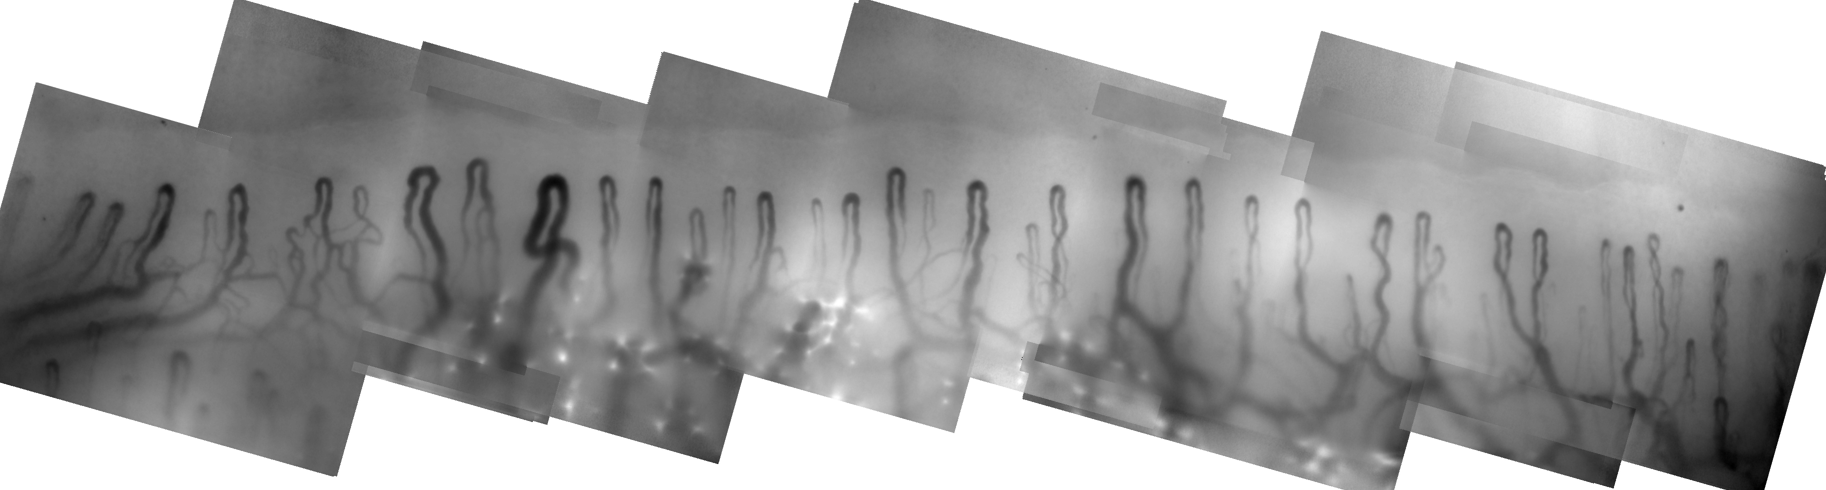
\includegraphics[width=0.98\columnwidth]{\figpath/nailfold_10598c} \\
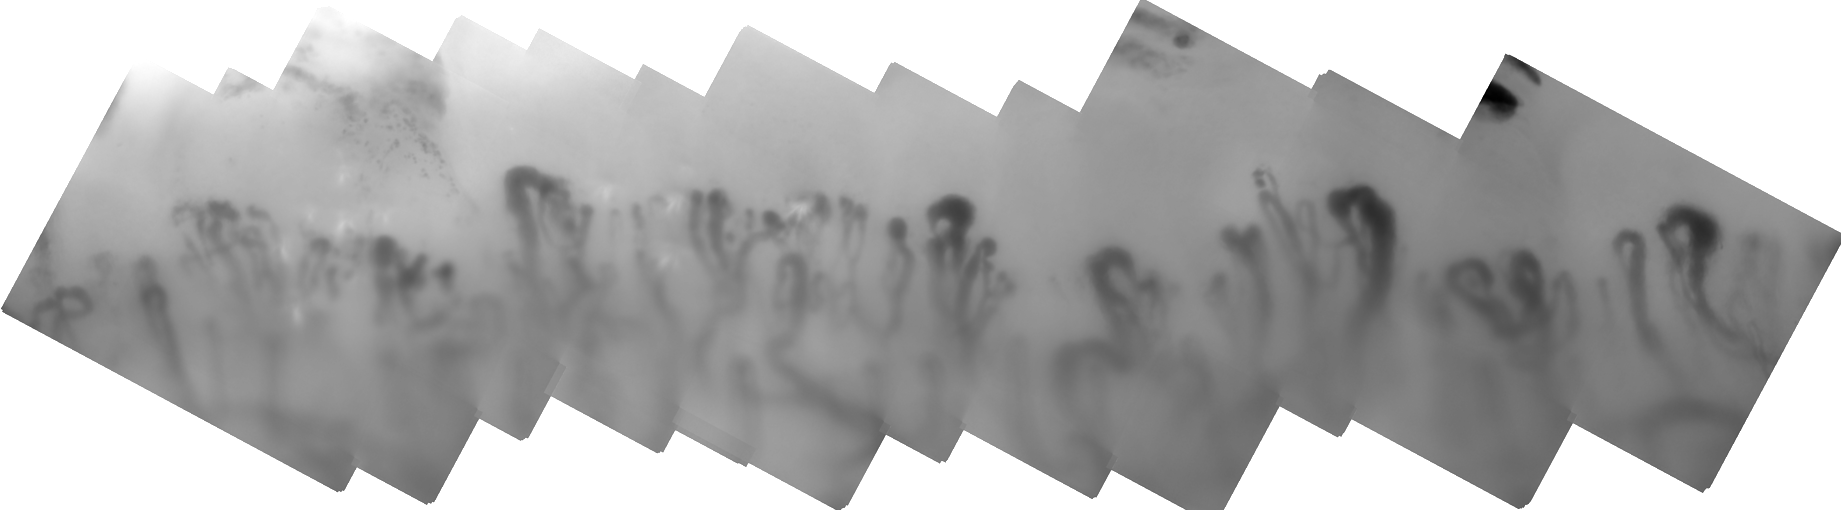
\includegraphics[width=0.98\columnwidth]{\figpath/nailfold_54611c} \\
\noalign{\smallskip}
\end{tabular}
%
\caption{Two example nailfolds}
\label{f:capillaroscopy}
\end{figure}
%
\section{Data}
The images used in this work were acquired by the capillaroscopy system in clinical use at Salford Royal Hospital Trust, UK. High magnification $768 \times 576$ pixel video frames are captured at a resolution of $12.5 \mu m$ per pixel. Sequential frames are compounded into a single static frame to provide as much contrast a possible to the capillaries. At this magnification only a fraction (typically about one fifth) of the nailfold is visible in each static frame, and thus the process is repeated at multiple horizontal locations. The frames are co-registered and stitched together to make a single image mosaic depicting the whole nailfold, as depicted in \fref{f:capillaroscopy}. Further details of this process are given in \cite{}.

The images are monochrome on an 8-bit grayscale. Masks separating the mosaic area from null background are automatically computed by finding all pixels with value 255 (\ie white) connected to the full rectangular image edge. These masks are then eroded by $X 50 \mu m$ so that spurious capillary detections at the edges of the mosaic are ignored. Throughout it is assumed that all further processing is applied only to pixels within the mosaic masks.

If the image mosaic has been correctly acquired, the capillaries should lie in a single, approximately horizontal row across the length of the image. These are referred to as distal capillaries. This spatial arrangement may be disrupted either by structural damage to microvasculature caused by SSc (evidence of which can be seen in the bottom mosaic of \fref{f:capillaroscopy}, or because of problems in the acquisition (typically mis-registrations where frames contain little to no contrast), noting also that the former may exacerbate the latter. Non-distal capillaries, typically situated below the main row, may also present and are not usually considered in manual assessment of the images.

We use a set of 990 image mosaics that have been manually annotated as part of an ongoing, separate clinical trial involving three subject groups: healthy controls (HC); subjects with primary Raynaud's phenomenon (PR); and patients with SSc. The images were annotated independently by two expert observers \footnote{note that the second observer for each image was not always the same person, but could have been one of a number of experts participating in the trial}. In each image, the observer attempted to mark the location and apical width of all distal capillaries, and mark the location of any other non-distal vessels. This is a challenging and inherently subjective task for which perfect agreement is rare, results for the agreement between markers are given in section \sref{s:results}.

In a subset of 80 images, observer one provided a precise demarcation of the inner and outer edges of the distal capillaries. Regions of interest about these capillaries were created a set of 450 training images with matching capillary masks, used to train vessel segmentation, orientation and width estimation in section \sref{s:segmenting_vessels} and the apex location predictors in section \sref{s:capillary_apexes}. The remaining images are split into a validation set of 456 images (104 HC, 83 PR, 269 SSc) used in sections \sref{s:capillary_apexes} and \sref{s:distal_row}, and a test set of 455 images (104 HC, 83 PR, 268 SSc) used in the results of section \sref{s:results}.

%
\section{Vessel segmentation, orientation and width estimation}
\label{s:segmenting_vessels}
From an image processing perspective, nailfold images contain a number of challenges: capillaries are often very low signal, particularly in SSc images were the microvasculature is damaged; the process of stitching the mosaic produces significant contrast changes across the image and may introduce artefacts where the frames are joined; finally,  due to the disease process, the size, shape, number and spacing of capillaries vary hugely throughout the data - for example, whilst the average width of a capillary is around $10-15 \mu m$, the largest can range up to $200-300 \mu m$.

As a result our detection models need to be robust to large changes in contrast, scale and rotation, without making fixed assumptions on the expected number of detections in an image. As a first step, we segment all blood vessels from background -- \ie we predict whether any given pixel in a nailfold image belongs to a vessel or vessel or the background. In addition we predict orientation and width of structure at each pixel, noting that such predictions only have sensible meanings at vessel pixels.

\subsection{Labelling images for machine learning}
We solve this as a machine learning task, training a classifier to perform segmentation and regressors for estimating orientation width. Segmentation via learning has become the preferred approach in similar tasks -- it allows the use of a complex set of features capable of characterising image structure without proscriptive assumptions on the values such features should take for specific data being used. A survey of all relevant methods is not feasible here, however the increase in performance of successive learning methods \cite{} over earlier analytical methods \cite{}in the segmentation of retinal blood vessels is an illustrative example. Choosing to regress estimations of width and orientation is less common ~\cite{Berks_etal_IPMI11}, but awards the same advantages over analytical estimations.

Learning requires a training set of images that have been manually annotated, such that each pixel has a binary label: background (0) or vessel (1). By skeletonising these binary masks to centreline pixels, we can then label each centreline pixel with its width (computing a distance transform to the negative of the full mask) and orientation (fitting a linear polynomial in $5\times5$ windows surrounding at each centreline pixel). Width and orientation labels are then expanded to the full vessel mask using a simple nearest pixel interpolation. Rather than training regressors solely on vessel pixels, we have found it beneficial to assign random values of orientation and width to background pixels and include these in the training data.

Note directly regressing an orientation $\theta$ in radians does not correctly deal with angle wraparound (orientations may be classed as far apart when they are, in fact, close together), a problem subsequently discovered in the method proposed in ~\cite{Berks_etal_IPMI11}. Instead we label orientation as a unit vector in the complex plane, $t = \cos 2\theta + i\sin 2\theta$, where doubling the angle $\theta$ makes orientation invariant to direction~\cite{Mardia_Jupp_00}. This permits a correct definition of variance for a set of orientations, the angular dispersion~\cite{Mardia_Jupp_00}, that is defined as the magnitude of the mean vector over the set \ie~$D = |(\sum{t_k})/N|$. This has a maximum of 1 when all $t_k$ are equal, and a minimum of 0 when orientations are distributed uniformly about the circle or when the sample consists of pairs exactly $180^\circ$ apart. Halving the inverse tangent of the mean vector returns the angular mean of the set in radians. %Since the dimension and threshold that define each split in a regression tree are typically chosen to maximise the sum of the variances of the two samples produced by the split, this correct measure ensures better splits within the tree structure and more accurate regression.

\subsection{Gaussian Derivative Features}
Next we define a feature vector to characterise the local structure at each training pixel, decomposing an image into responses of symmetric (even) and asymmetric (odd) filters across scale and orientation. Like several previous methods we use directional second order derivatives of a Gaussian kernel for the even filters \cite{}. \footnote{Throughout, we use $G \equiv G(x,y;\sigma)$ to refer to a 2-dimensional Gaussian kernel with zero mean and standard deviation $\sigma$, and use subscripts to denote derivatives of $G$ with respect to a particular direction. We define the image responses to any filter $G_i{ij}$ as $I_{G_{i,j}}$.} At a given scale $\sigma$, three separable basis filters -- $\Gxx$, $\Gyy$ and $\Gxy$ -- can be steered to compute the equivalent response to a filter at any arbitrary angle $\theta$ ~\cite{Freeman_Adelson_TPAMI91,Koenderink_vanDoorn_TPAMI92,Karssemeijer_teBrake_TMI96}:

%
\begin{equation}
I_{G_\theta} = \Ixx \cos^2(\theta) + \Iyy \sin^2(\theta) + \Ixy \sin(2\theta),
\label{e:secondderivs_response}
\end{equation}
%
However, as recommended in the earlier work of ~\cite{Freeman_Adelson_TPAMI91} we supplement the even filters with their Hilbert transform, using four separable basis filters
%
\begin{equation}
H_a = 0.9780(2.2540x + x^3)G
\label{e:secondderivs_hilberta}
\end{equation}
\begin{equation}
H_b = 0.9780(0.7515 + x^2)yG
\label{e:secondderivs_hilbertb}
\end{equation}
\begin{equation}
H_c = 0.9780(0.7515 + y^2)xG
\label{e:secondderivs_hilbertc}
\end{equation}
\begin{equation}
H_d = 0.9780(2.2540y + y^3)G
\label{e:secondderivs_hilbertd}
\end{equation}
%
to generate a steered response
\begin{align}
   I_{H_\theta} = ~~~ &I_{H_a} \cos^3(\theta) \nonumber \\
   								 -~ &I_{H_b} 3\cos^2(\theta)\sin(\theta) \nonumber \\
   								 +~ &I_{H_c} 3\cos(\theta)\sin^2(\theta) \nonumber \\
   								 -~ &I_{H_d} \sin^3(\theta).
\label{e:secondderivs_hilberts}
\end{align}
%
At an initial scale $\sigma=1$ we compute responses $Igt$ and $\Iht$ at six angles $\theta_i = \nicefrac{i\pi}{6}$. We then compute responses at an additional four scales, in each case keeping $\sigma$ fixed whilst downsampling the image by a factor of 2 in each direction before upsampling the responses to original resolution via bilinear interpolation (thus the coarsest scale is equivalent to $\sigma=16$ at the original image resolution).

At each pixel the responses centred at that pixel, along with its 8-connected neighbours, are concatenated into a feature vector without further manipulation. Note that previous methods have suggested trying to analytically estimate the dominant direction, and then producing rotation invariant features by rearranging orientation responses about this direction. Whilst this may seem like an elegant method of obtaining a more compact feature space, in practice we have found that due to the errors in the analytical estimation of orientation this offers no benefit and may even reduce performance. Further details of experiments to justify these choices are provided in the supplementary material.

\subsection{Random Forests}
We train three random forests, one classifier on the binary background versus vessel lables, and a regressor each for the orientation and width labels. Each forest contains 100 trees. Rather than bootstrapping from a fixed sample of data, we sample a new set of 100k background and 100k vessel pixels from the set of images to train each tree (although the same set maybe reused for each of the three forests). For efficiency, the raw separable filters $G_xx$, $H_a$ \etc are applied once to the images and stored. The upscaled, steered responses can then be computed for the pixels included in the sample for each tree. We also maintain maps of which pixels were selected for each tree, so that unbiased predictions can be made on the training images for use in the next section.

Throughout $\sqrt{D}$ of the $D$ dimensions in the feature vectors are tested for splitting. The standard Gini coefficient is used to determine splits and stopping criteria in the classification trees, whilst for regression trees we maximise the sum of the variances of the two samples produced by the split (where, as noted above, we use the angular dispersion for orientation variance).

To make predictions in an unseen image we apply the separable basis filters, compute the interpolated, steered responses and extract feature vectors, before feeding the vectors through the trees in each forest and computing the mean pooled over all leaf nodes as the prediction output (applying the latter four stages block-by-block for large images). For orientation, the unit vectors are converted back to radians. The result for each input image is a map of vessel segmentation ($V_p$), orientation ($V_\theta$) and width ($V_w$).

\section{Locating Candidate Capillaries}
\label{s:capillary_apexes}
The vessel segmentations (\ie pixels with values in $V_p$ close to 1) should contain the capillaries we are looking for, however they will also contain other structures that aren't capillaries. Some of these are due to imperfections in the trained classifier, however even in perfect conditions it is inevitable that structures such as larger blood vessels (often found near the bottom of images, but not always present) will be segmented as their local appearance is indistinguishable from enlarged capillaries. Thus the next step in our method is to find candidate locations in the segmented vessels for the apices of individual capillaries.

As training data we use the segmentation, orientation and width prediction maps for the same training images used in the previous section, where the output for each pixel is computed using only those trees in which that pixel wasn't an input training sample.

First the vessel probability maps are thinned by applying non-maximal suppression in conjunction with the orientation maps. That is a pixel $q = (x,y)$ is kept if and only if
%
\begin{equation}
V_{nms}(x,y) =
\begin{cases}
V_p(x,y)   & \mbox{if } V_p(x,y) > \max \left( V_p(x \pm n_x, y \pm n_y) \right) \\
0          & \mbox{otherwise }
\end{cases}
\label{e:nms}
\end{equation}
%
where $n_x = \cos(V_\theta(x,y))$ and $n_y = \sin(V_\theta(x,y))$, and sub-pixel values of $V_p$ are computed via bilinear interpolation.

Next we define a base width $W$ as the median vessel width sampled at each of the capillary apexes in the training set. Then for each positive pixel $q$ in $V_{nms}$ we extract a $64 \times 64$ patch from $V_p$ centred at $q$, scaled by $\nicefrac{W}{V_w(p)}$ (where the initial spacing is at the original image resolution) and rotated by $V_\theta(q)$.

If a patch about $q$ contains a capillary apex and $q$ is also a vessel pixel in the original training masks, then the patch is labelled positive and the offset to the apex (relative to the coordinate frame of the patch, not the original image) is recorded  -- otherwise the patch is labelled as negative. In this manner multiple positive patches are associated with each apex.

For each patch a histogram of gradients (HoG)  feature vector is formed by concatenating histograms of gradient direction weighted by gradient magnitude in each of the 64 $8 \times 8$ blocks~\cite{HoG}. Following the guidance in \cite{HoG}, 9 orientation bins are used for each block, and the weighted gradient of each pixel is interpolated over neighbouring bins. However we found normalising the histograms gave no benefit, most probably due to the fact the values of $V_p$ are already mapped to $[0, 1]$.

A 100 tree random forest classifier is then trained to distinguish between positive and negative patches, whilst a regression forest is trained to predict the offset associated with each positive patch. This time, due to the limited amount of positive data, we take bootstrap samples for each tree (although the negative samples in the classifier can still be sub-sampled without replacement from the complete data if desired).

For an unseen image, having computed $V_p$, $V_\theta$, $V_w$ and $V_{nms}$, we extract scale and rotation normalised patches about each positive pixel in $V_{nms}$ and pass these through the classification forest. The output labels at each leaf node are pooled and averaged, forming $\alpha(q)$, the probability that the patch about $q=(x,y)$ contains an an apex. The regression forest is then used to predict the offset $(u,v)$ to the nearest apex, which is then rescaled and rotated (using the inverse of the transform used to extract the patch) to locate the prediction $a = (x+u',y+v')$ in the original image coordinate frame. A Gaussian kernel centred at $a$, scaled by $V_w(a)$ and weighted by $\alpha(q)$ is added to a vote map of apex locations $A$. The local maxima of $A$ are then used as candidate locations for capillary apexes.

In practice we have found it beneficial to apply a threshold $\lambda$ to the weights $\alpha(q)$, thus ignoring the offset votes for any $q$ where $\alpha(q) < \lambda$. \fref{f:capillaroscopy} shows detection performance as a function of $\lambda$, suggesting value of approximately $\lambda = ?$ is suitable. The figure also show performance where the offset votes are not weighted by $\alpha(q)$, again as a function of threshold $\lambda$, clearly showing the benefit of weighting. We also tried a scheme in which each tree votes individually (as used in \cite{}), however we found this increased the number of false positives without any increase in sensitivity.

Note that in addition to the usual advantage of regression voter over straightforward classification -- that of aggregating information from multiple patches to determine each candidate location -- we get have the additional advantage that candidate locations are not restricted to lying on the pixels in $V_nms$. Thus we benefit from the efficiency of only computing features and predictions for a greatly reduced number of pixels but can still predict apices anywhere in the vicinity of a vessel centreline.

\section{Selecting Distal Capillaries}
\label{s:distal_row}
As shown in fig ?, even in the best scenario, the initial capillary apex candidates comprise many false positives. In this section we aim to reduce these in two ways: firstly we reclassify each candidate, now using only the locations of apex candidates as positive and negative training data; secondly we exploit the spatial constraints inherent in the image format and specifically the fact that the capillaries should lie in a single, approximately horizontal line across the image. As part of the latter step, in addition to discarding false positives, we separate distal from non-distal vessels (the latter being candidates with strong capillary appearance, but located outside -- and usually below -- the distal row).

As data, we use candidate apexes computed for the set of 441 validation images. Each candidate $C_i=(x_i,y_i)$ is labelled as positive if it was marked by either observer (where the tolerance about each observer apex is a circle with diameter equal to the apical width marked by the observer) and negative otherwise, giving approximately X positive and Y negative samples. The positive samples are further split into X distal and Y non-distal capillaries.

\subsection{Rescoring Capillary Appearance}
\label{s:distal_appearance}
A classifier is trained as before using a random forest of 100 trees, taking bootstrap bootstrap samples of positive and negative samples for each tree, and using HoG features on scale and rotation normalised patches extracted about each sampled candidate. However we now extract patches from the original grayscale image, having found this works better than using $V_p$. The output of the trees are pooled to give a single appearance score between $0$ and $1$ for each candidate, allowing us to define each candidate as the tuple of its location and score, $C_i=(x_i,y_i,c_i)$. A detection ROC for the set of $C_i$ from all images in the validation set is shown in fig .

Using a classifier here may seem contrary to the claims at the end of \sref{s:capillary_apexes}, however the key difference between this and the earlier classification is that we are now able to focus explicitly on differentiating capillary apexes and artefacts in the background with a similar (but noticeably different to a human observer) appearance. Attempting this classification directly, when the negative class includes all possible background patches results in significantly worse performance. However focusing classification solely on candidates returned from regression voting means that $c_i$ is significantly better at separating positive and negative candidates than $A(x_i,y_i)$, as shown in the marginal distributions in figure F.
%
\begin{figure}[t]
\centering
\begin{tabular}{@{}c c c@{}}
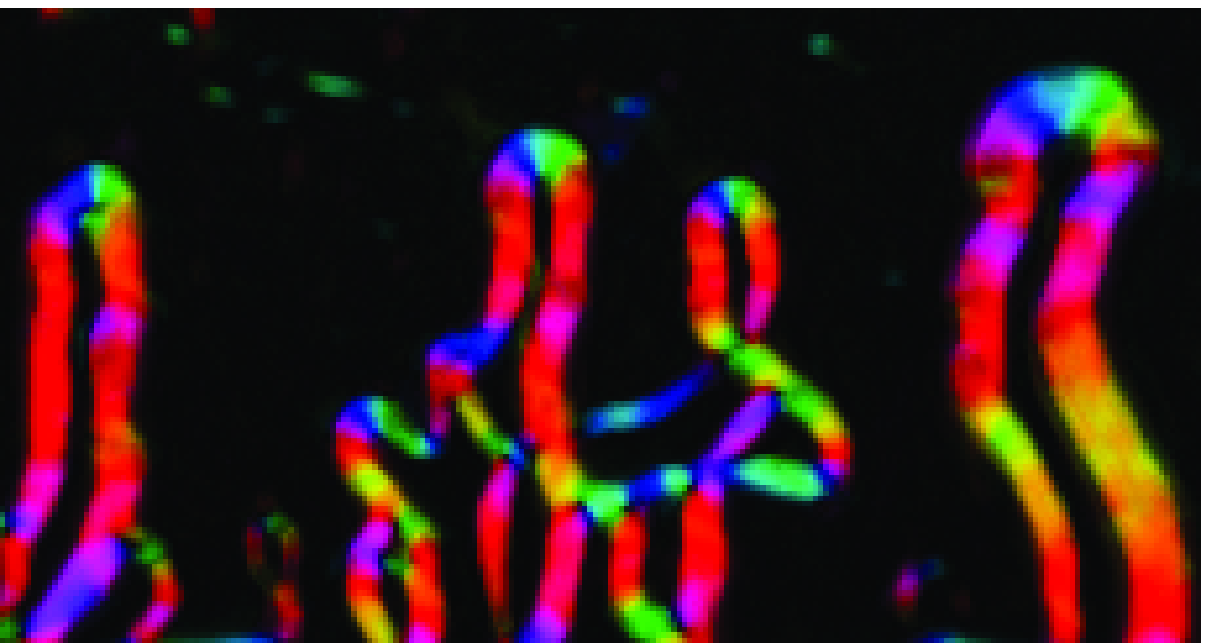
\includegraphics[width=0.31\columnwidth]{\figpath/02_orientation_prediction} &
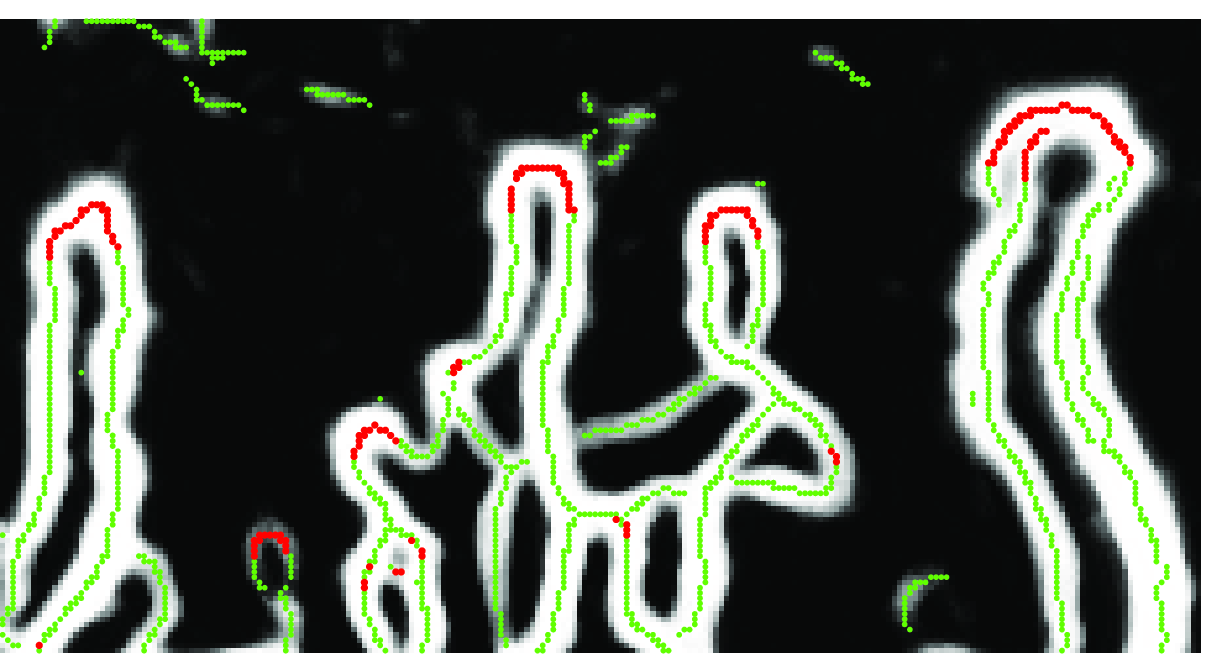
\includegraphics[width=0.31\columnwidth]{\figpath/01_vessel_prediction} &
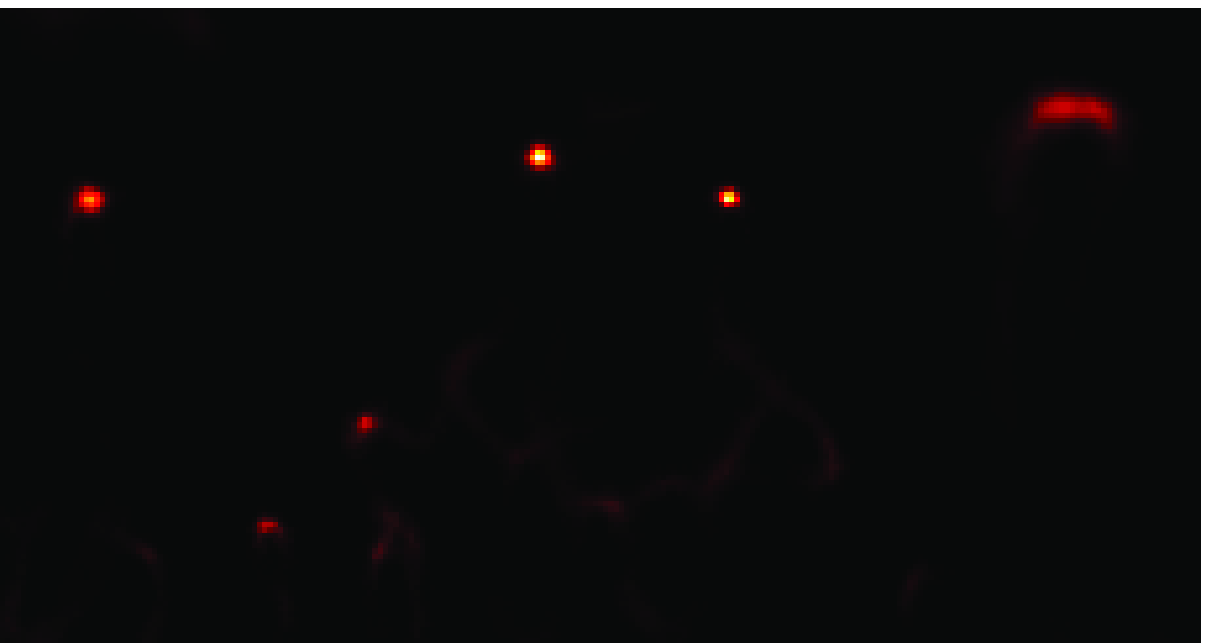
\includegraphics[width=0.31\columnwidth]{\figpath/03_apex_heat_map} \\
(a) & (b) & (c)\\
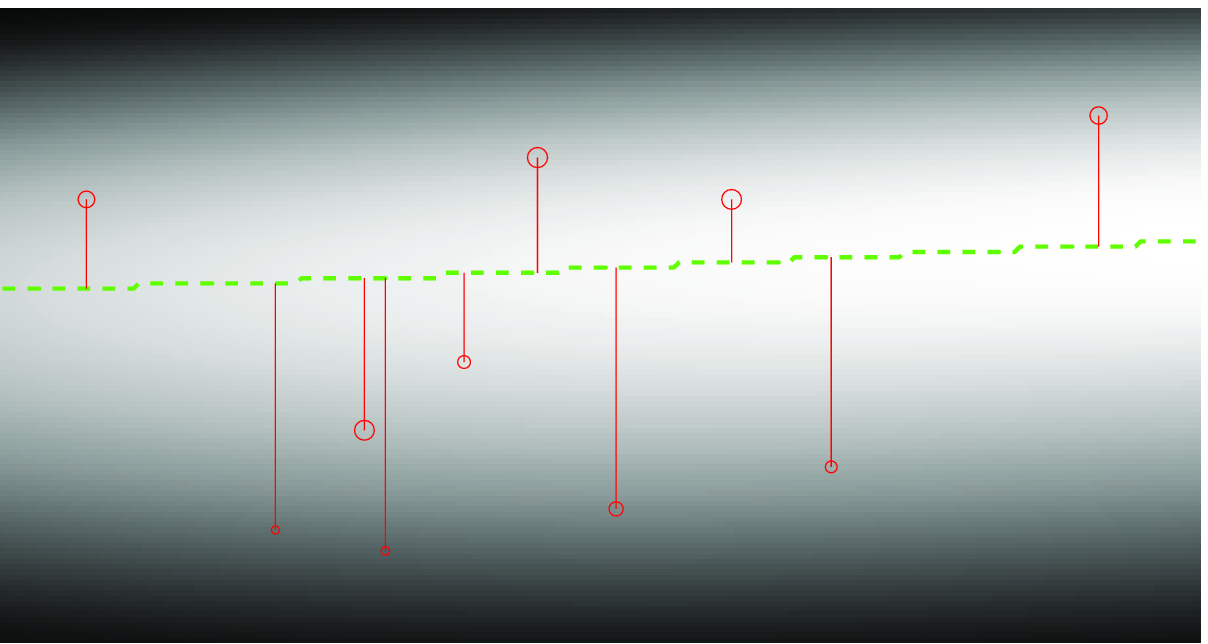
\includegraphics[width=0.31\columnwidth]{\figpath/04_apex_location_map} &
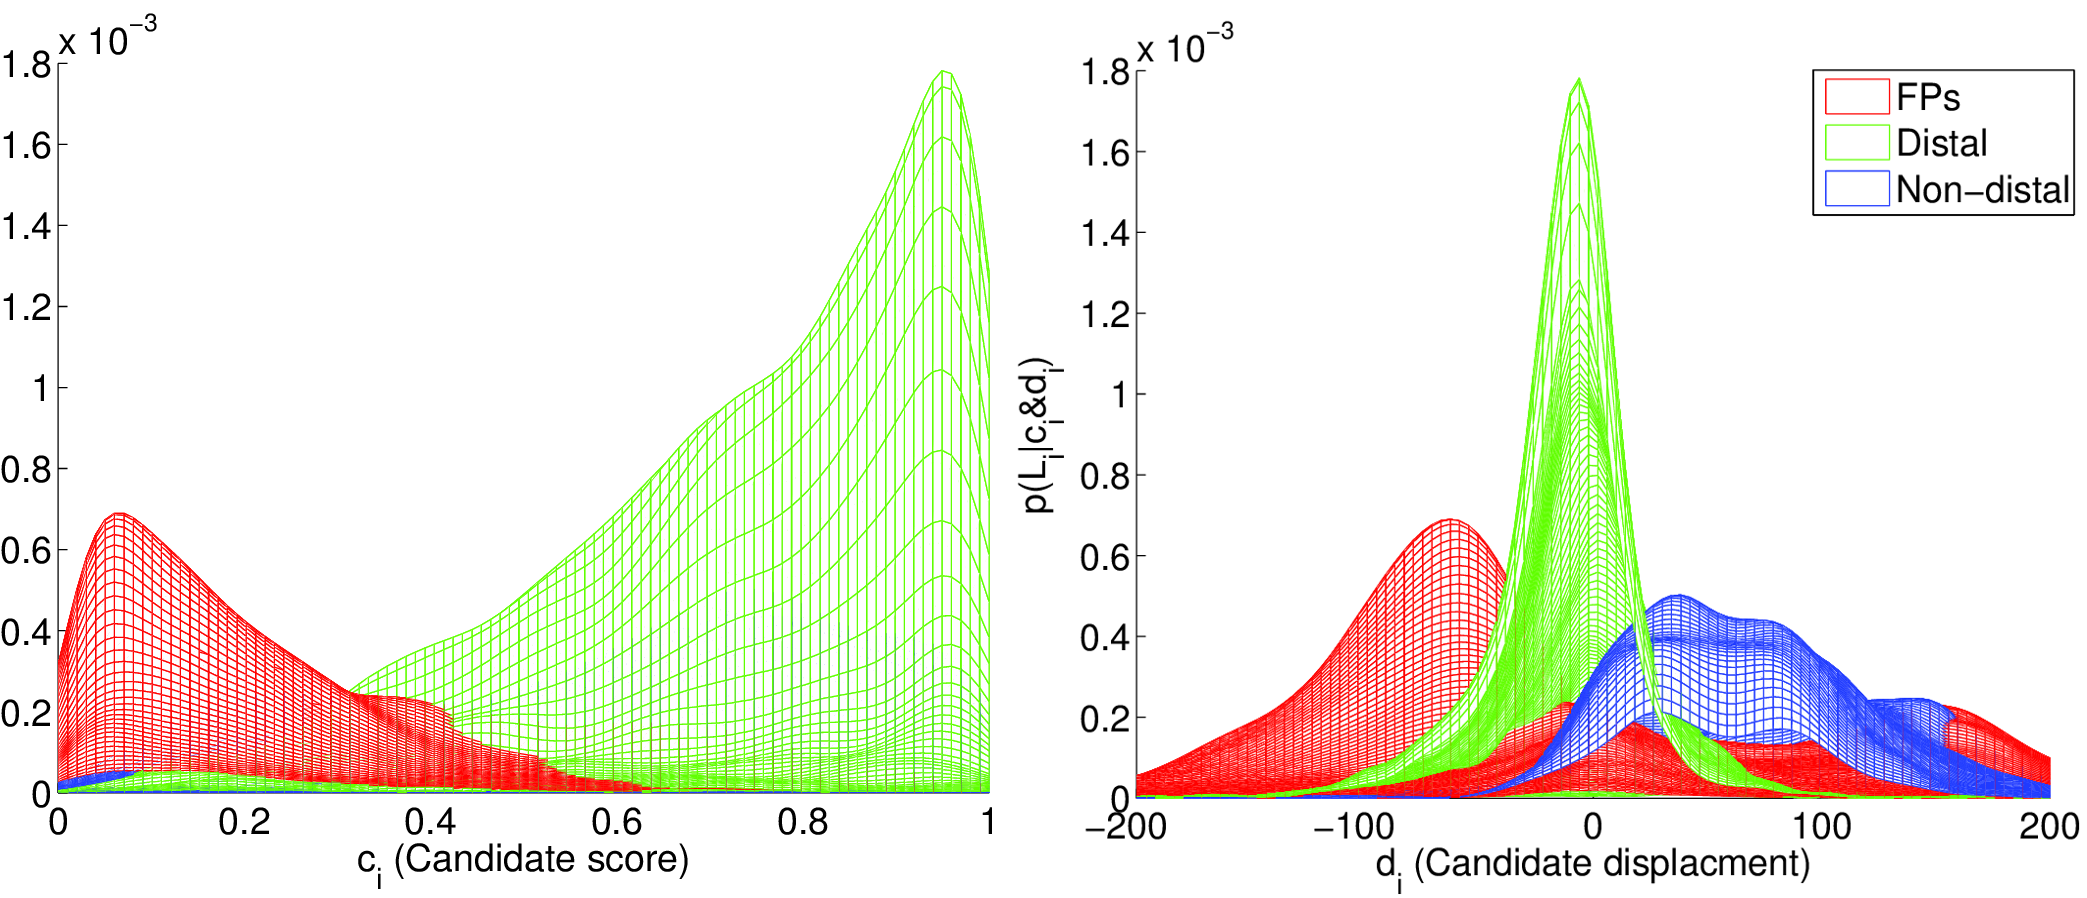
\includegraphics[width=0.31\columnwidth]{\figpath/05_conditional_pdfs} &
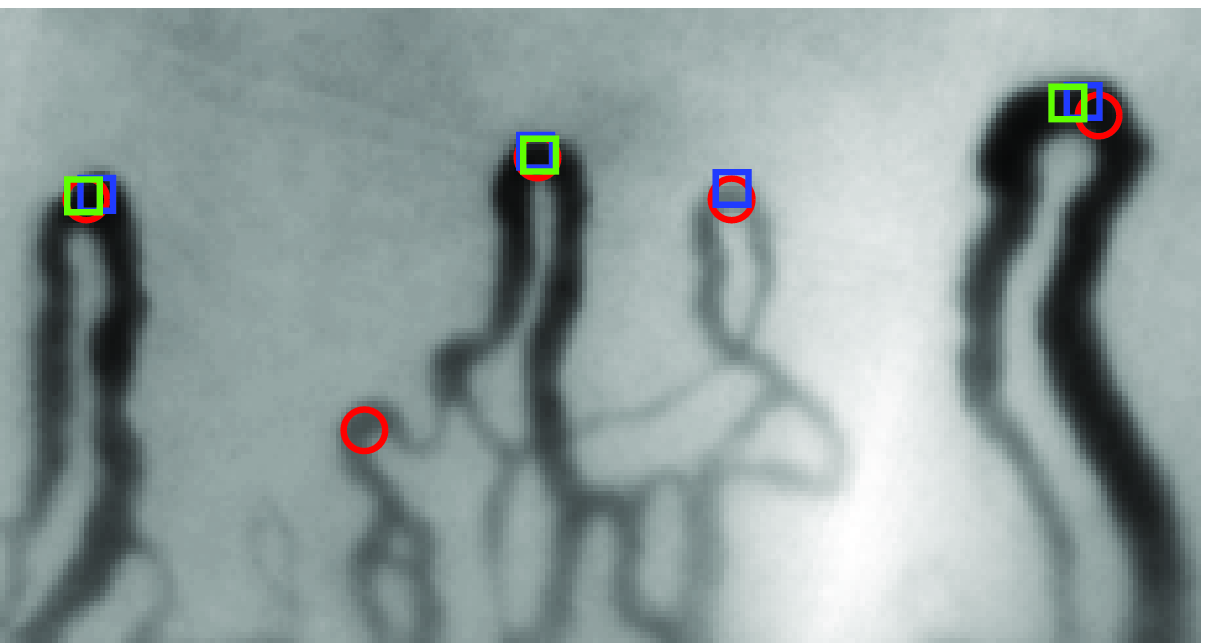
\includegraphics[width=0.31\columnwidth]{\figpath/00_nailfold} \\
(d) & (e) & (f)\\
\noalign{\smallskip}
\end{tabular}
%
\caption{Estimating orientation in retinography: %
(a) ; %
(b);%
(c);%
(d);%
(e);%
(f);%
}
\label{f:capillaroscopy}
\end{figure}
%
\subsection{Capillary Location}
\label{s:distal_location}
In addition to the final appearance score, the location of a candidate relative to the other candidates in any image provides useful information on its likelihood of being a distal row apex. If we assume the ideal distal row to be some approximately smooth non-parametric line running across the full width of the image mosaic passing through each true capillary apex, then if this line can be estimated in an unseen image, we can compute the vertical displacement of each candidate to the line.

To achieve this, we compute a density map of candidate locations by summing a Gaussian kernel centred at each discrete candidate location. Each kernel is weighted by the candidate's appearance score, so that strong candidates contribute more to the density. The density for each location in the mosaic can thus be computed as
%
\begin{equation}
D(u,v) = A\sum\limits_{i=1}^N c_i\exp \left[ -\frac{(u-x_i)^2}{2{\sigma_x}^2}\right]\exp \left[ -\frac{(v-y_i)^2}{2{\sigma_y}^2}\right]
\label{e:kernel_estimate}
\end{equation}
where there are $N$ candidates in the image, and $A$ is a normalisation constant so that $D$ sums to unity. Values for $\sigma_x$ and $\sigma_y$ are computed following the method described by Hall \cite{} such that
%
\begin{equation}
\sigma_x = 1.06N^{\nicefrac{-1}{5}} \left[ (N-1)^{-1} \sum\limits_{i=1}^N (x_i - \bar{x})^2 \right] ^{\nicefrac{1}{2}}
\label{e:kernel_sigma}
\end{equation}
%
Substituting $y$ for $x$ produces an equivalent formula for $\sigma_y$. As in \sref{s:capillary_apexes}, performance is improved in the candidates a thresholded by their score, so that only those with $c_i > 0$ contribute to $D$.

$D$ is used to compute the vertical displacement from each candidate to the maximum of $D$
%
\begin{equation}
d_i = y_i -  \operatorname*{arg\,max}_v D(x_i,v)
\label{e:candidate_displacment}
\end{equation}
%
Using the ground truth, each candidate in the validation images $C_i=(x_i,y_i,c_i,d_i)$ is also assigned a label $l_i \in [1,2,3]$ for false positives, distal capillaries and non-distal capillaries respectively. Figure ? shows a kernel estimate of the class-conditional probability density $P(c_i, d_i | l_i)$. The class priors for each label type $P(li)$ can be empirically estimated from the data, and thus we can use a standard Bayes rule transormation to compute the probability of each candidate belonging to a class, given its appearance score and displacement
%
\begin{equation}
d_i = y_i -  \operatorname*{arg\,max}_v D(x_i,v)
\label{e:candidate_displacment}
\end{equation}
%

\section{Results}
\label{s:results}
Vessel detection...

Bootstrap samples of the test set to compute error bars.

Co-occurrence matrix between observer one, observer two and the automated method.

A vs B

\% A distal missed by B = 36.8

\% A distal marked as distal by B = 55.5

\% A distal marked as non-distal by B = 7.68

---

B vs A

\% B distal missed by A = 22

\% B distal marked as distal by A = 77.7

\% B distal marked as non-distal by A = 0.298

-----------------------------------------------------------------

A vs C

\% A distal missed by C = 20.2

\% A distal marked as distal by C = 74.1

\% A distal marked as non-distal by C = 5.76

---

C vs A

\% C distal missed by A = 47.8

\% C distal marked as distal by A = 104

\% C distal marked as non-distal by A = 5.72

-----------------------------------------------------------------

A vs C

\% A distal missed by C = 20.2

\% A distal marked as distal by C = 74.1

\% A distal marked as non-distal by C = 5.76

---

C vs A

\% C distal missed by A = 30.4

\% C distal marked as distal by A = 66

\% C distal marked as non-distal by A = 3.64

-----------------------------------------------------------------

B vs C

\% B distal missed by C = 20.5

\% B distal marked as distal by C = 76.7

\% B distal marked as non-distal by C = 2.82

---

C vs B

\% C distal missed by B = 44.7

\% C distal marked as distal by B = 48.8

\% C distal marked as non-distal by B = 6.5

-----------------------------------------------------------------

%
\begin{table}[tb]
\centering
%\small
\input{cooccurrence_table.txt}
%
\caption{Caption here.}
\label{t:cooccurrence}
\end{table}
% 
\begin{table}[tb]
\centering
%\small
\input{cooccurrence_table2.txt}
%
\caption{Caption here.}
\label{t:cooccurrence_marginals}
\end{table}
% 

Apex measurement: subject group distributions for vessel density

%
\begin{figure}[t]
\centering
\begin{tabular}{@{}c c c@{}}
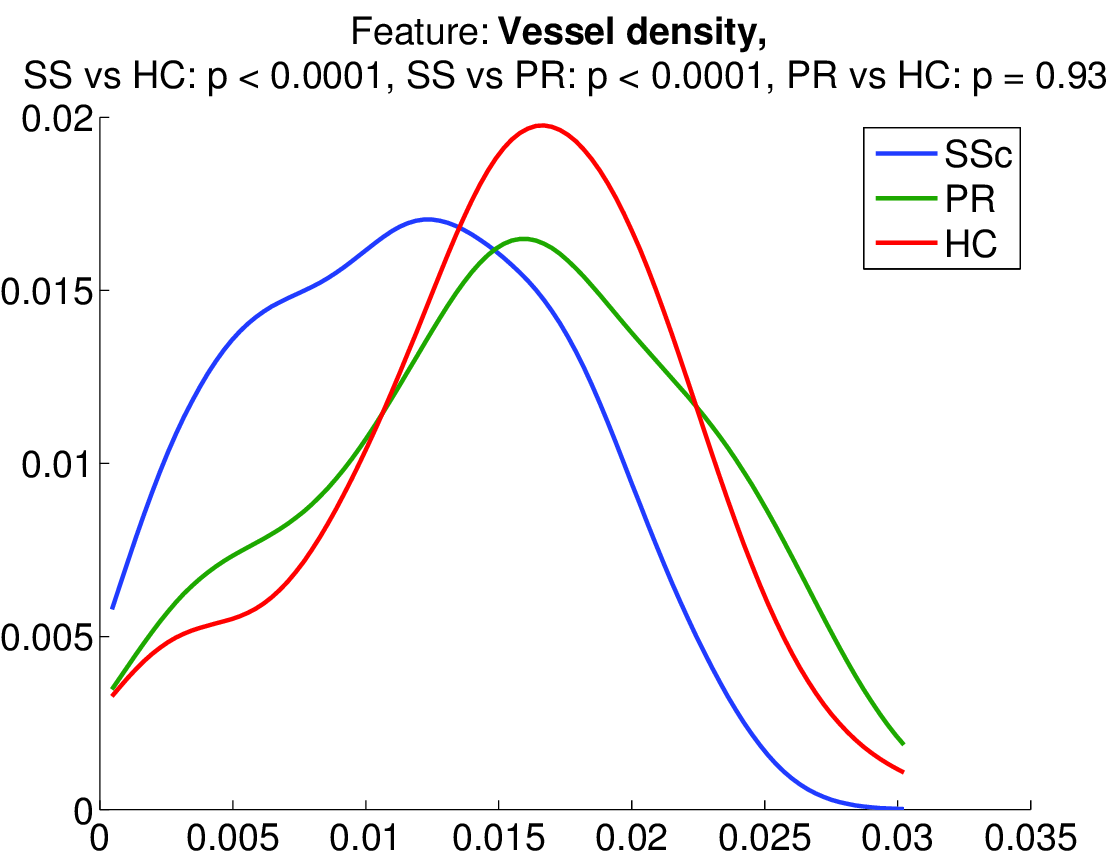
\includegraphics[width=0.31\columnwidth]{\figpath/vessel_density_pdf} &
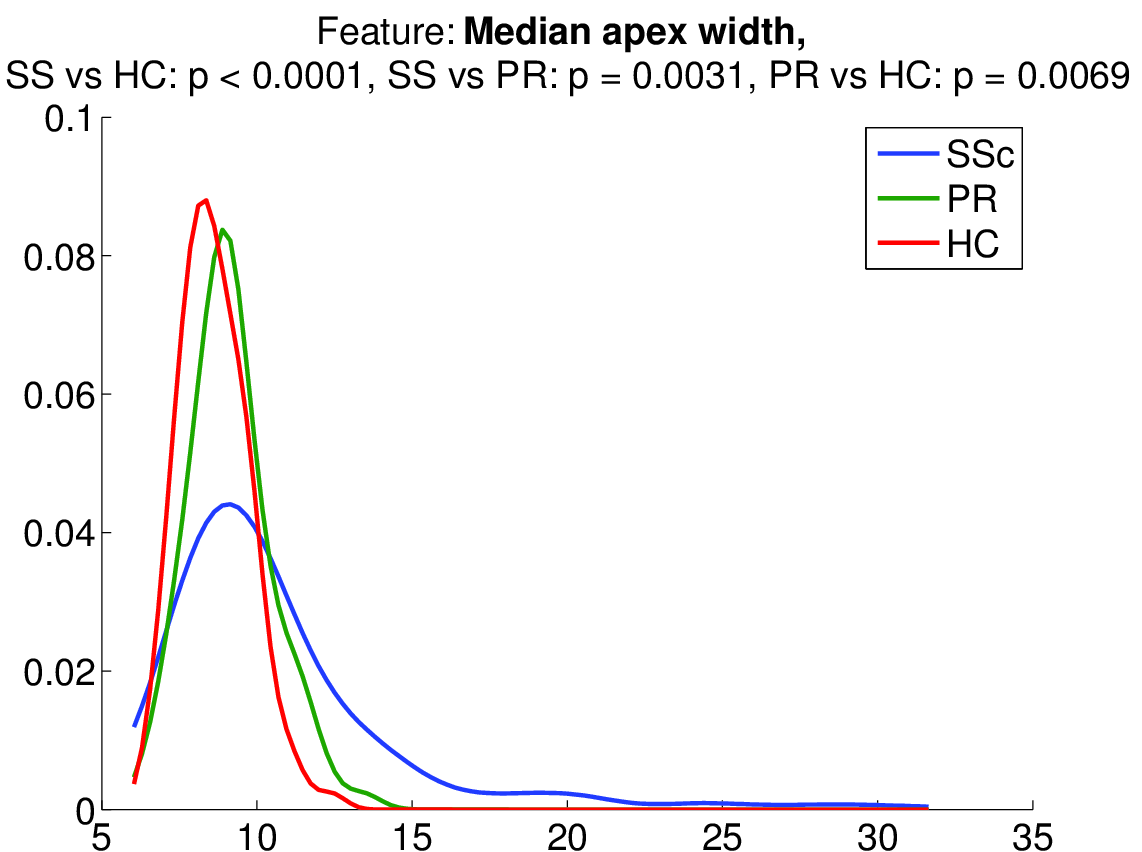
\includegraphics[width=0.31\columnwidth]{\figpath/median_apex_width_pdf} &
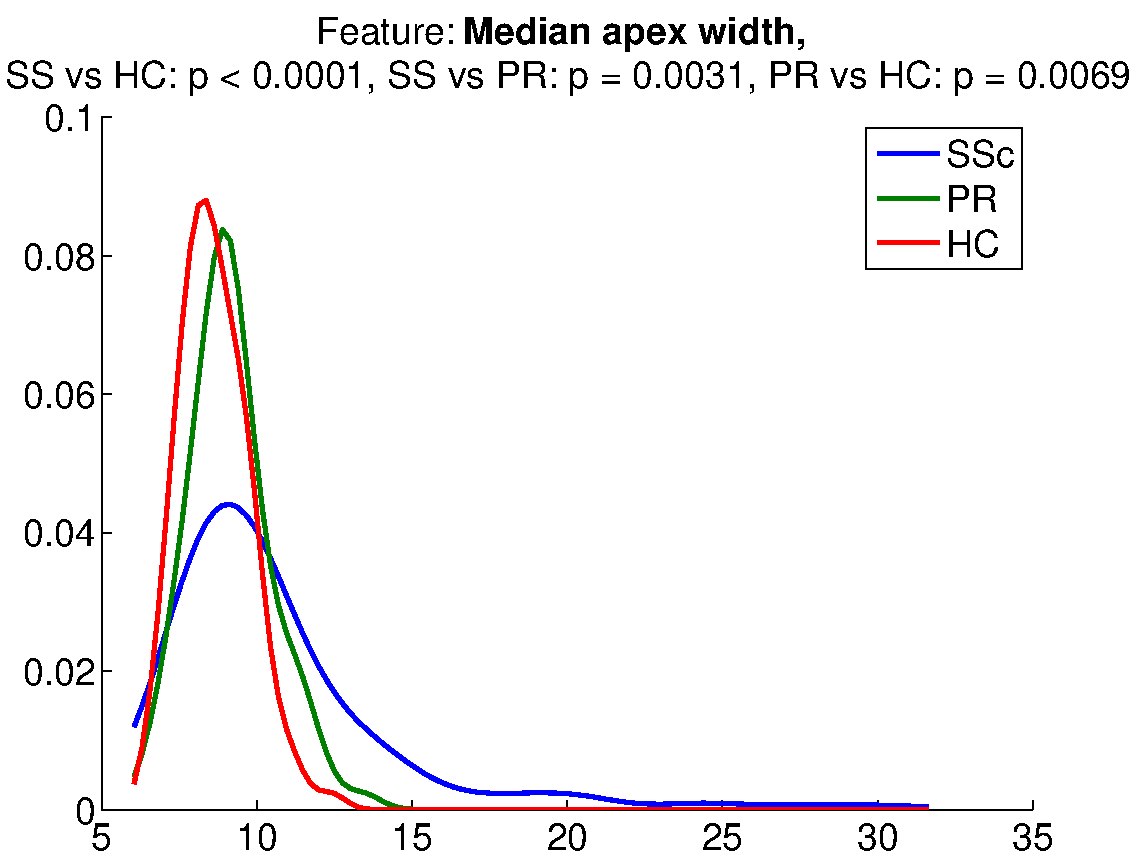
\includegraphics[width=0.31\columnwidth]{\figpath/median_orientation_entropy_pdf} \\
(a) & (b) & (c)\\
\noalign{\smallskip}
\end{tabular}
%
\caption{Estimating orientation in retinography: %
(a) ; %
(b);%
(c);
}
\label{f:subject_apex_measures}
\end{figure}
%

\section{Conclusions}
\label{s:conclusions}
It was good.

%\end{document}

\bibliographystyle{splncs}
\bibliography{./bib/_aliases,./bib/mobio,./bib/mammography,./bib/ml,./bib/local,./bib/nailfold}

\end{document}
